\subsection{Policies}
\label{subsec:policies}

In our empirical application\comment[id=K]{Improve language} we distinguish four groups
of contact types: households, education, work and other contacts.% households
For households we assume that the individuals'
contacts in their households do not change over our estimation period.
% educ models
For nurseries, preschools and schools we implement vacations as announced by the German
federal states as well as school closures, emergency care and A / B schooling where only
one half of students attends every other week or day. For the moment we ignore that lack
of childcare leads working parents to stay home. An approximation of the share of contacts still taking place with the different school regulations can be found in Figure~\ref{fig:school_multiplier}.

\begin{figure}
    \centering
    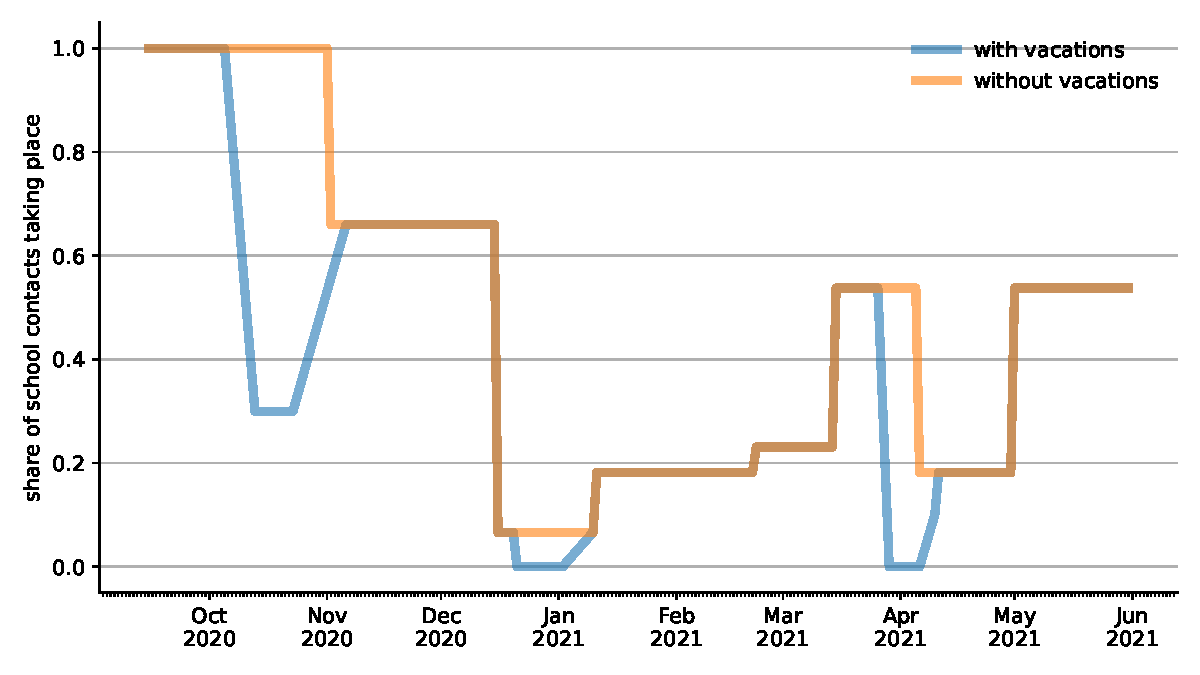
\includegraphics[width=\textwidth]{figures/results/figures/data/school_multiplier_comparison}
    \caption{School Multiplier With and Without Vacations Factored In}
    \floatfoot{\noindent \textit{Note:} The dates on which schools have vacation are
    decided at the federal level. Vacations are directly implemented in our model with no
    school contacts taking place on weekends and during vacations (by federal state) just
    like the schooling mode (full operation, emergency care, rotating schemes with half
    class sizes etc.). The figure is thus only an illustration that roughly shows the
    share of contacts taking place compared to pre-pandemic level with and without
    vacations. The difference between the lines show when vacations take place and to
    what degree. For example all states have fall vacations but the timing varies
    strongly between states.}
    \label{fig:school_multiplier}
\end{figure}


%
% Schließung von Kindertagesstätten und Schulen: 37,4 Millionen ausgefallene Arbeitstage
% http://www.iab-forum.de/schul-und-kitaschliessungen-krankheit-quarantaene-die-coronabedingten-arbeitsausfaelle-der-erwerbstaetigen-steigen-auf-592-millionen-arbeitstage/
%
%
% https://www.sueddeutsche.de/politik/schulschliessung-lockdown-bildung-1.5190377: In
% allen Ländern geht trotz des Lockdowns ein erheblicher Anteil der Schülerinnen und
% Schüler in die Schule.
% https://gfx.sueddeutsche.de/apps/e525337/www/_image_desktopw1840q70-1e2e2bf78b7d4430
% 18% der Grundschüler in Notbetreuung in BW
%

% work
For our work contacts we use the reductions in work mobility reported in the Google
Mobility Data \citep{Google2021} to calibrate our work policies. Reductions in work
contacts are not random but governed through a work contact priority where the policy
changes the threshold below which workers stay home. Figure \ref{fig:work_multiplier}
shows the share of workers that go to work in our model over time.

\begin{figure}[ht]
    \centering
    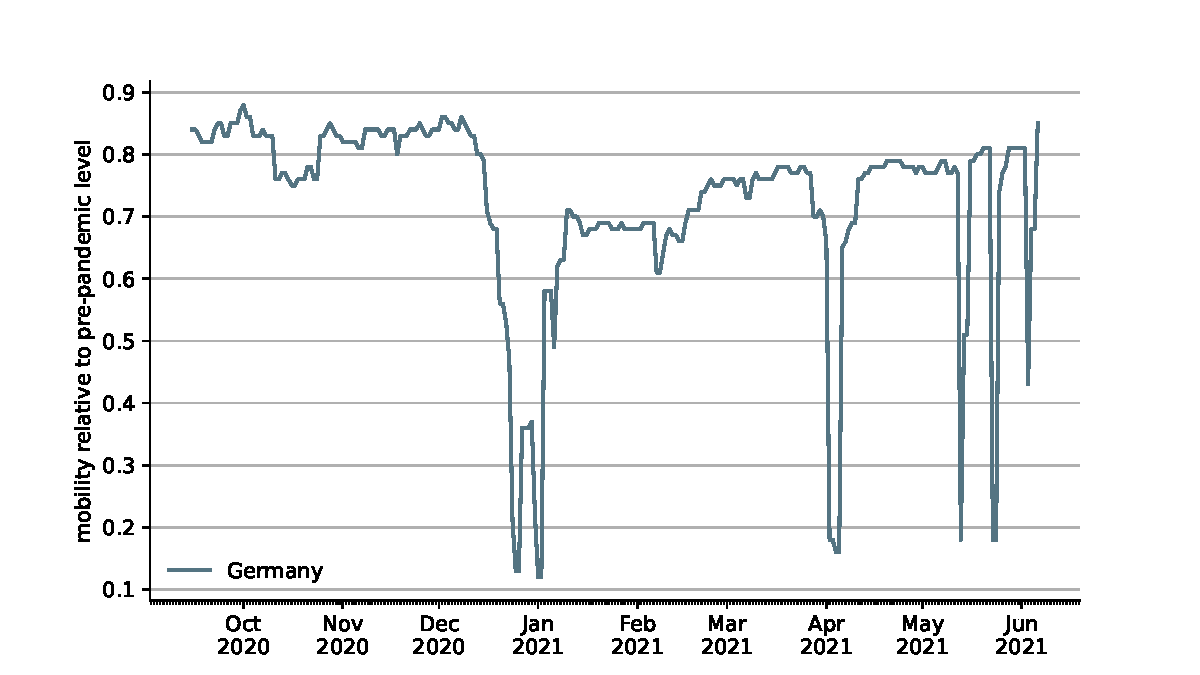
\includegraphics[width=\textwidth]{figures/results/figures/data/work_multiplier_since_sep}
    \caption{Share of Workers with Work Contacts}
    \label{fig:work_multiplier}
    \floatfoot{\noindent \textit{Note:} The figure shows the work mobility as reported by
        \cite{Google2021}. We take this as a proxy of the share of workers who are not in
        home office, i.e. who still have physical work contacts. The figure interpolates
        over weekends as we handle weekend effects through information on work on
        weekends in the German census data we use. The figure shows the share aggregated
        over Germany as a whole. To capture the effect that local policies, school
        vacations and public policies have on work contacts we use the data on the level
        of the federal states to determine which workers go to work depending on the
        state they live in.}
\end{figure}

For both work and school contacts we assume that starting November with the lockdown
light in Germany, hygiene measures (such as masks, ventilation and hand washing) became
more strict and more conscientiously observed, leading to a reduction of 33\% in the
number of contacts with the potential to transmit Covid-19.

For the last group of contacts, which cover things like leisure activities, grocery
shopping, etc., we have no reliable data by how much policies reduce them. In addition,
they are likely to be affected by social and psychological factors such as pandemic
fatigue and vacations. Because of this we estimate them like the infection probabilities
to fit the time series data. We use very few change points and tie them to particular
events such as policy announcements or particular holidays. Because of the scarce data
situation we cannot distinguish between a hygiene factor (such as mask wearing) during
meetings and physical distancing (such as virtual meetings with
friends).\comment[id=K]{@Janos: Maybe make more concrete when the estimation is finished
which phases we have and why the switching points are where they are.}

\begin{figure}
    \centering
    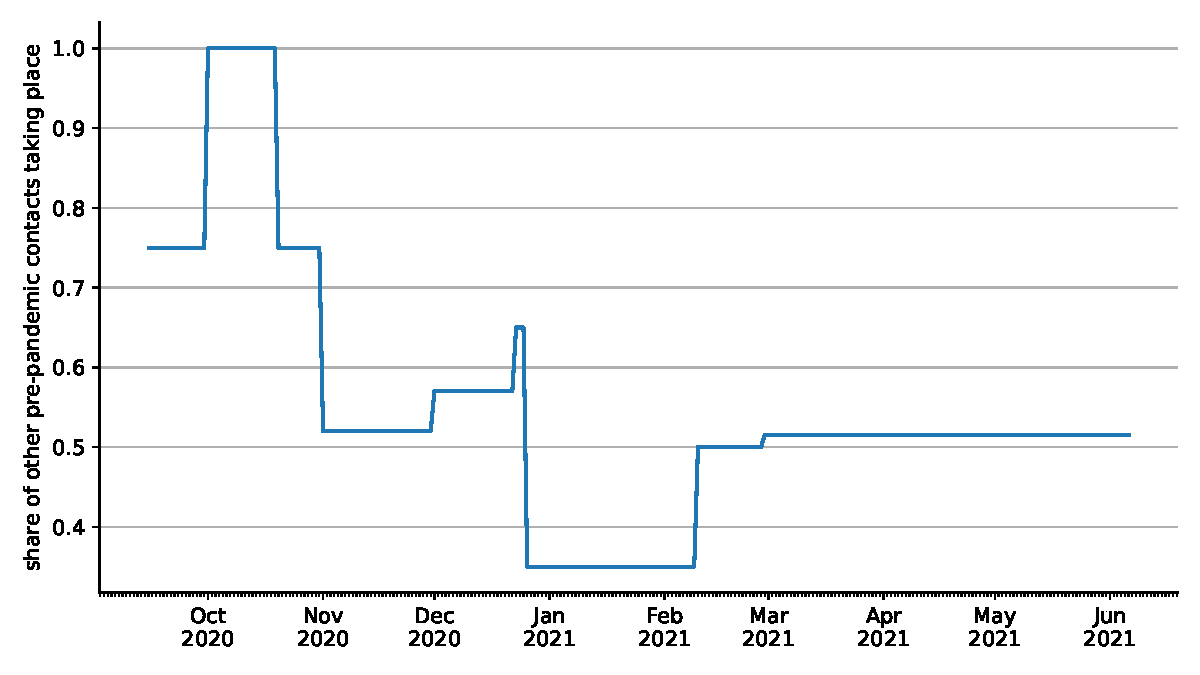
\includegraphics[width=\textwidth]{figures/results/figures/data/other_multiplier}
    \caption{Share of Pre-Pandemic Other Contacts Taking Place with Infection Potential}
    \label{fig:other_multiplier}
    \floatfoot{\noindent \textit{Note:} All values are estimated. We try to use as little
    switching points as possible and tie them to political events (such as lockdown
    announcements) unless changes are used to capture anticipation or pandemic fatigue
    (for example we model an anticipation of the November lockdown and model lockdown
    fatigue in early March).}
\end{figure}

\FloatBarrier

